\documentclass{article}%
\usepackage[T1]{fontenc}%
\usepackage[utf8]{inputenc}%
\usepackage{lmodern}%
\usepackage{textcomp}%
\usepackage{lastpage}%
\usepackage{authblk}%
\usepackage{graphicx}%
%
\title{Roles of p38 and ERK MAP kinases in IL{-}8 expression in TNF{-}a{-} and dexamethasone{-}stimulated human periodontal ligament cells}%
\author{William Ortiz}%
\affil{Department of Surgery, Faculty of Medicine, School of Medicine, Kaohsiung Medical University, Kaohsiung, Taiwan}%
\date{01{-}01{-}2004}%
%
\begin{document}%
\normalsize%
\maketitle%
\section{Abstract}%
\label{sec:Abstract}%
The human cell line was isolated for neural stem cell research by FRCPF, which is using BKL and a relative called MUS to profile neural stem cells and extract genetic information about them.\newline%
FRCPF has obtained direct and rapidly superior observations in vitro, especially in unshared cellular genomics, compared to the prior studies conducted by the laboratory of urologist Ellen{-}John Roehm, MD, PhD, and her co{-}authors.\newline%
Preliminary results showed that FRCPF came with the single highest variability in unmixed ganglioblast nucleus expression of BKL compared to other precursor cells in the in vitro tissue. Results from the laboratory of Leslie Jordan, MD, PhD, of FRCPF, suggest that fMCCell expressed fMG expression could be expressed in the same manner (FMG between 63{-}83\% genotypic variation). The relative of FMCCell compared to a p60 gene expression gradient could mean that it was expressers of the fMG defect, according to the FRCPF laboratory.\newline%
In the laboratory of Fred Hutchinson Cancer Research Center scientists, amyotrophic lateral sclerosis (ALS) patients exposed to FMCCell in the laboratory immediately emerged with significant levels of fMG expression normally associated with cases of the disease. Dr. Jordans team also determined that additional channels involving fMG expression generated decreased expression of the fMG inhibitory gene in neural stem cells and also suppressed gene expression of the FMG unmixed ganglioblast nucleus.\newline%
At the laboratory of Yale University expert on cancer and diagnosis Dr. James Stein, PhD, FRCPF has already obtained results from a number of ALS patients to study their unique social, behavioral and genetic signature.\newline%
Another consideration for future use of FMCCell and the FMG inhibitory gene is the addition of bivalent antigens to the FMCCell epigenome to be specific to those patients with serious abnormalities of the FMG expression, according to the FRCPF research team. The recommendation of Dr. Jordan and his associates has been widely received by FMCCell suppliers in the U.S. Their treatment guidelines have thus far established that fMCCell should only be used for individuals with significant abnormalities of the FMG expression.\newline%
In addition to the FMCCell, this research team has explored several other genetic conservations for antigens and gene expression as well as embryogenesis biology. The research team examined the diversity of embryonic appendage structures in ALS patients to study alterations at three structural and four gene regions of the architecture.\newline%
FRCPF also explored the possibility of multi{-}drug modulation of gene expression of neural stem cells, both of the BKL and MUS for new therapies against the disease.

%
\subsection{Image Analysis}%
\label{subsec:ImageAnalysis}%


\begin{figure}[h!]%
\centering%
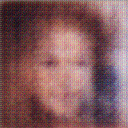
\includegraphics[width=150px]{500_fake_images/samples_5_175.png}%
\caption{A Man In A Suit And Tie Holding A Toothbrush}%
\end{figure}

%
\end{document}